
\documentclass{article}

% if you need to pass options to natbib, use, e.g.:
%     \PassOptionsToPackage{numbers, compress}{natbib}
% before loading neurips_2018

% ready for submission
% \usepackage{neurips_2018}

% to compile a preprint version, e.g., for submission to arXiv, add add the
% [preprint] option:
\usepackage[preprint]{neurips_2019}

% to compile a camera-ready version, add the [final] option, e.g.:
     % \usepackage[final]{neurips_2019}

% to avoid loading the natbib package, add option nonatbib:
%     \usepackage[nonatbib]{neurips_2018}

\usepackage[utf8]{inputenc} % allow utf-8 input
\usepackage[T1]{fontenc}    % use 8-bit T1 fonts
\usepackage{hyperref}       % hyperlinks
\usepackage{url}            % simple URL typesetting
\usepackage{graphicx}
\usepackage{booktabs}       % professional-quality tables
\usepackage{amsfonts}       % blackboard math symbols
\usepackage{nicefrac}       % compact symbols for 1/2, etc.
\usepackage{microtype}      % microtypography
\usepackage{listings}
\usepackage{tabularx}
\usepackage{listings}
\usepackage{pgfplots}
\usepackage{tikz,pgf}
\usepackage{todonotes}
\usepackage{tikz-cd}
\usepackage{algorithm}
\usepackage{algpseudocode}
\usepackage{wrapfig}
\usepackage{amsmath,amsthm}
\usepackage{amssymb}
\tikzset{>=latex}
\usetikzlibrary{bayesnet}
\usetikzlibrary{arrows,shapes,automata}
\usetikzlibrary{positioning}
\newcommand{\n}[1]{\ensuremath{n_{#1}}}
\newcommand{\rv}[1]{\ensuremath{{#1}_{1:n_{#1}}}}
\newcommand{\rvv}[1]{\ensuremath{{#1}_{1:n_{#1'}}}}
\newcommand{\model}[1]{\ensuremath{\mathcal{M}{(#1)}}}
\newcommand{\simu}[1]{\ensuremath{\Omega(\model{#1})}}
\newcommand{\micro}[2]{\ensuremath{\phi_{#1}(#2)}}
\newcommand{\pdf}[1]{\ensuremath{\mathcal{P}_{d}(#1)}}
\newcommand{\pmf}[1]{\ensuremath{\mathcal{P}_{m}(#1)}}
\newcommand{\add}[1]{\ensuremath{A_{#1}}}
\newcommand{\adds}[2]{\ensuremath{A_{#1}_{#2}}}
\newcommand{\expect}[1]{\ensuremath{\mathbb{E}[#1]}}
\newcommand{\trace}[1]{\ensuremath{\mathcal{T}_{#1}}}
\newcommand{\traces}[2]{\ensuremath{\textit{tr}^{#1}_{#2}}}
\newcommand{\stoc}[2]{\ensuremath{f^{#1}_{#2}(\rvv{x})}}
% \usepackage[binary-units=true]{siunitx}
\title{Hijacking Simulators with Universal Probabilistic Programming}

% neurlps classification
% Primary: Applications
% Secodnary cat:Data, Challenges, Implementations, and Software
% or Hijacking Malaria Simulators with Probabilistic Programming

% The \author macro works with any number of authors. There are two commands
% used to separate the names and addresses of multiple authors: \And and \AND.
%
% Using \And between authors leaves it to LaTeX to determine where to break the
% lines. Using \AND forces a line break at that point. So, if LaTeX puts 3 of 4
% authors names on the first line, and the last on the second line, try using
% \AND instead of \And before the third author name.
\newcommand{\bg}[1]{~{{[{\it \textcolor{red}{{\bf BG:} #1}}]}}}
\newcommand{\cs}[1]{~{{[{\it \textcolor{red}{{\bf CS:} #1}}]}}}
\newcommand{\ag}[1]{~{{[{\it \textcolor{red}{{\bf AG:} #1}}]}}}
% If accepted, instead use the following line for the camera-ready submission:
%\usepackage[accepted]{icml2019}

\lstset{language=C++,
                basicstyle=\footnotesize,
                keywordstyle=\color{blue}\ttfamily,
                stringstyle=\color{red}\ttfamily,
                commentstyle=\color{green}\ttfamily,
                morecomment=[l][\color{magenta}]{\#},
                breaklines = true
}
\pgfplotsset{width=7cm,compat=1.8}
\author{%
Paper ID: 1010 }
  % examples of more authors
  % \And
  % Coauthor \\
  % Affiliation \\
  % Address \\
  % \texttt{email} \\
  % \AND
  % Coauthor \\
  % Affiliation \\
  % Address \\
  % \texttt{email} \\
  % \And
  % Coauthor \\
  % Affiliation \\
  % Address \\
  % \texttt{email} \\
  % \And
  % Coauthor \\
  % Affiliation \\
  % Address \\
  % \texttt{email} \\
%}
\begin{document}
% \nipsfinalcopy is no longer used

\maketitle

\begin{abstract}

    Notes on how to develop a formalism to perform inference in population based simulators.
\end{abstract}

\section{Introduction}
\label{sec:intro}

One challenge in performing inference in such models is the combinatorial increase in \emph{paths}
that can be taken within the given probabilistic model.
This is because each member of the population has 
a bounded, but large number of decisions to make. 
In addition to this, each member of the population can interact
with other members of the population.
To model a single population member quantum-based methods leveraging 
linear superposition and entanglement provide an ability to explore multiple paths simultaneously maintaining 
the whole program, \emph{state}, in one iteration.
 Unfortunately, analytically writing the functional 
form of the state is, in this instance, impossible.   
The usability of current classical inference methods in this context is also problematic. 
However, by combining hijacking and amortizing parts of the simulator, in particular rejection sampling 
loops, we can not only correctly perform inference in such models, as the rejection sampling loops are 
now replaced with learnt functions, but we can also perform inference much more efficiently. 
This is because the rejection sampling loops are now replaced with learnt functions which enables us to correctly
construct the density and as they are amortized, evaluation is cheap and only has to be performed once per call.
This significantly reduces memory consumption and running time. 


Without the amortization procedure, as updates are made sequentially MCMC methods are typically not-well suited this type of recursive
estimation problem. 
As each time we get a new data point $y_{t+1}$ we have to run new MCMC simulations 
for $P(x_{0:t_1}| y_{0:t+1})$, we also cannot directly reuse the samples $\{x^{i}_{0:t}\}$. 
However, as we can only run the simulator $\texttt{forward()}$ we cannot return back to a previous state and re-run. 
So adapting existing inference techniques is the only viable option. 
MCMC methods can be effective with a well designed amortized inference procedure (\textbf{Note: This is not guaranteed}).
Non-MCMC based methods such as importance sampling (IS) and sequential monte carlo (SMC), may also be
sensible inference engines, although we shall discuss the limitations within the simulator context in the proceeding sections.  

However, to implement this in practice we are required to do the following:
 \begin{itemize}
    \item Create a sensible training procedure
    \item Have 2 additional functions implemented within pyprob
    \begin{enumerate} \item 1) That stores only the necessary raw samples from the desired rejection sampling addresses to be used for training.
                       \item 2) A function at \emph{test time} that replaces those given addresses with a learnt surrogate.
    \end{enumerate}
    \item Finer grained control over the actual latent variables of interest, to avoid unnecessary memory consumption and ensure that inference problems remain tractable.
  \end{itemize}
There is no doubt that implementing some fo these features will be more invasive to the underlying simulator code than previously
just hijacking the raw-random number draws, but, it would enable us to attack difficulties in the inference procedures that are
currently not amenable to the current approach.

 % !TEX root = notes.tex

\tikzset{
    state/.style={
           rectangle,
           rounded corners,
           draw=black, very thick,
           minimum height=2em,
           inner sep=2pt,
           text centered,
           },
}

\begin{figure}
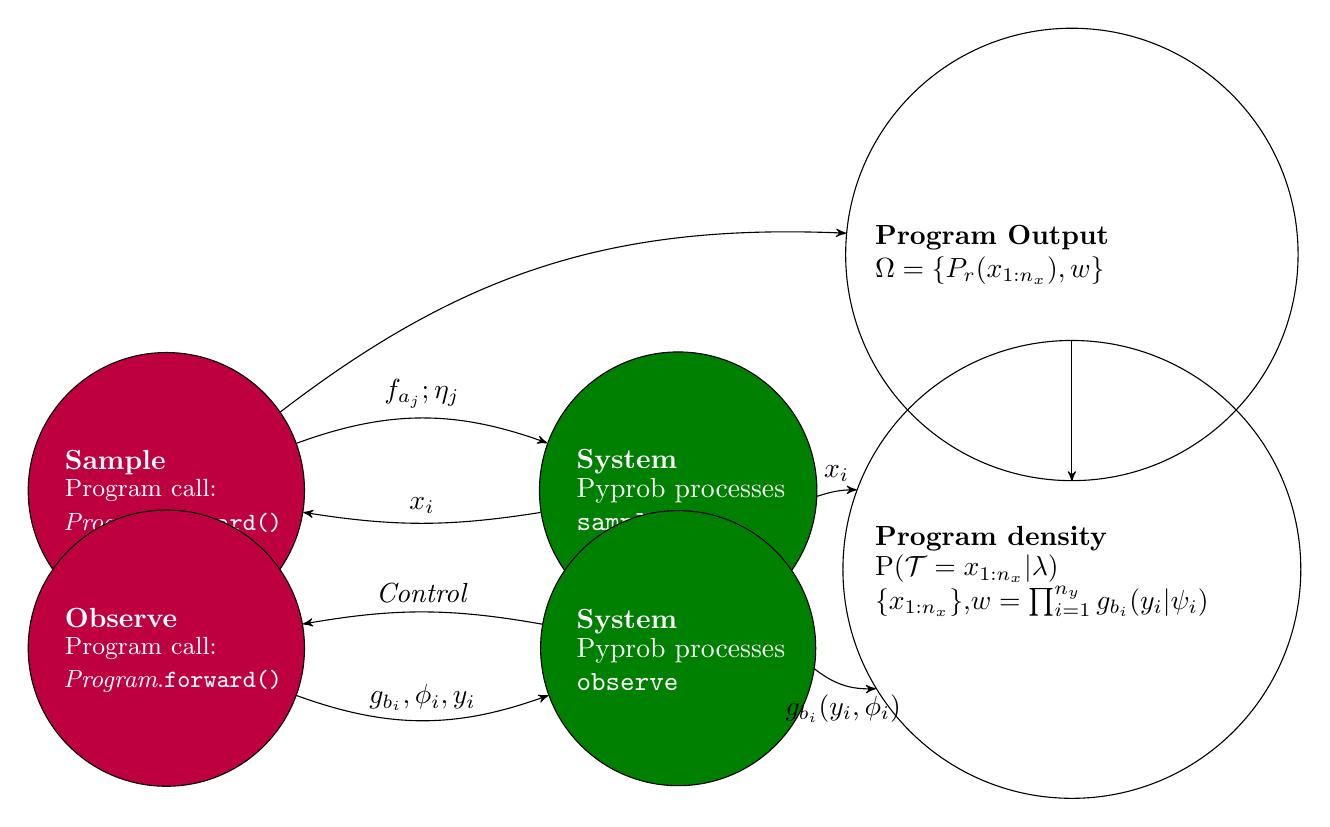
\begin{tikzpicture}[->,>=stealth']

 % Position of Sample 
 % Use previously defined 'state' as layout (see above)
 % use tabular for content to get columns/rows
 % parbox to limit width of the listing
 \node[state,
 text width=3cm, 	% max text width
 yshift=0cm, 		% move 2cm in y
 node distance=0cm, 	% distance to Sample
 anchor=center,
 fill=purple] (Sample) 
{%
\begin{tabular}{l} 	% content
  \textcolor{white}{\textbf{Sample}}\\
  \parbox{4cm}{
  \textcolor{white}{\small{Program call:\\
  \emph{Program}.\texttt{forward()}}}
 }
 \end{tabular}};
  
 \node[state,    	% layout (defined above)
 text width=3cm, 	% max text width
 yshift=-2cm, 		% move 2cm in y
 below of=Sample, 	% Position is to the right of Sample
 node distance=0cm, 	% distance to Sample
 anchor=center,
 fill= purple] (OBSERVE) 	% posistion relative to the center of the 'box'
{%
\begin{tabular}{l} 	% content
  \textcolor{white}{\textbf{Observe}}\\
 \parbox{4cm}{
  \textcolor{white}{\small{Program call:\\
  \emph{Program}.\texttt{forward()}}}
}
\end{tabular}};

 % State: PyProb with different content
 \node[state,    	% layout (defined above)
  text width=3cm, 	% max text width
  yshift=0cm, 		% move 2cm in y
  right of=Sample, 	% Position is to the right of Sample
  node distance=6.5cm, 	% distance to Sample
  anchor=center,
  fill = black!50!green] (PyProb) 	% posistion relative to the center of the 'box'
 {%
 \begin{tabular}{l} 	% content
  \textcolor{white}{\textbf{System}}\\ %system sample
  \parbox{4cm}{\textcolor{white}{Pyprob processes\\ \texttt{sample}}}
 \end{tabular}
 };
 
 % STATE System
 \node[state,
  below of=PyProb,
  yshift=-1cm,
  anchor=center,
  text width=3cm,
  fill = black!50!green] (System) 
 {%
 \begin{tabular}{l}
  \textcolor{white}{\textbf{System}}\\
  \parbox{4cm}{\textcolor{white}{Pyprob processes \\\texttt{observe}}}
 \end{tabular}
 };

 % STATE EPC
 \node[state,
  right of=System,
  yshift = 1cm,
  node distance=5cm,
  anchor=center] (EPC) 
 {%
 \begin{tabular}{l}
  \textbf{Program density}\\
  \parbox{5cm}{P($\mathcal{T}= x_{1:n_x}| \lambda)$\\
  \{$x_{1:n_{x}}\}$,$w= \prod^{n_{y}}_{i=1} g_{b_i}(y_i | \psi_i)$}
 \end{tabular}
 };


  % STATE OUTPUT
  \node[state,
  above of=EPC,
  yshift = -1cm,
  node distance=5cm,
  anchor=center] (OUTPUT) 
 {%
 \begin{tabular}{l}
  \textbf{Program Output}\\
  \parbox{5cm}{$\Omega = \{P_{r}(x_{1:n_{x}}), w\}$}
 \end{tabular}
 };

 % draw the paths and and print some Text below/above the graph
 \path (Sample) 	edge[bend left=20]  node[anchor=south,above]{$f_{a_{j}} ; \eta_{j}$}(PyProb)
 (OBSERVE)     	edge[bend right=20] node[anchor=south,above]{$g_{b_{i}},\phi_i , y_i $} (System)
 (System)       	edge [bend right=20] node[anchor=south,below]{$g_{b_{i}}(y_i, \phi_i)$} (EPC)
 (PyProb)       edge [bend left=9] node[anchor=west, above]{$x_{i}$} (Sample)
 (PyProb)       edge [bend left=9] node[anchor=west, above]{$x_{i}$} (EPC)
%  (System)       	edge [bend left=10]                                          (EPC)
 (EPC)              edge                                                    (OUTPUT)
 (System)  	edge [bend right=10]  node[anchor=north,above]{\emph{Control}} (OBSERVE)
 (Sample)   edge [bend left= 20] (OUTPUT) ;
%  (System)  	edge[loop below]    node[anchor=north,below]{$SC_n\neq 0$} (System)
%  (System)  	edge                node[anchor=left,right]{$SC_n = 0$} (PyProb);

\end{tikzpicture}
\caption{An overview of the hijacking system. $x_i$ represent latent variables. $f_{a_i}$ represent raw sample calls,
$g_{b_j}$ represent conditioning statements. $\mathcal{T}$ corresponds to the program trace. $w$ represents the collective weights. 
$r$ represents run number. $n_x$ represents the number of latent variables and $n_y$ represents the number of
observations, which will always be fixed, but is model dependent. $\lambda$ represents all the other variables generated 
by running the simulator \texttt{.forward()}.
}
\label{fig:systemoverview}
\end{figure}
\section{Limitations with different inference engines}  

\subsection{Prior based sampling}
In prior based sampling we take our existing program and look directly at the product of all the raw sample calls, denoted $f_{a_i}(x_i | \eta)$ and 
construct a proposal that is is dependent on those. In this sampling scheme our proposal is defined as:
\begin{equation}
  q(x_{1:n_{x}}) = 
  \begin{cases}
    \prod_{i=1}^{n_x} f_{a_i}(x_i | \eta) \hspace{0.1cm} \texttt{if} \hspace{0.1cm} \mathcal{B}(x_{1:n_{x}})=1 \\
    0
  \end{cases}
\end{equation}
where $\mathcal{B}(\cdot)$ is satisfied by the simulator and $f_{a_i}(\cdot)$ represents a
raw random sample, $\eta$ is a subset of the variables in-scope at the point of sampling
and $n_{x}$ is the number of latent variables.
 This is true in all inference engines used in this hijacking framework.
However, this makes use of no conditioning and is not sufficient for performing inference in
complex, population-based simulations.


\section{Non-prior Based Sampling}
In non-prior based sampling we utilise conditioning too, which enables 
us to explore spaces more efficiently. 
In the current hijacking set-up, we
can only do conditioning at the end of each \texttt{forward()} run of the simulator. 
This does inhibit certain inference engines and makes aspects of performing inference 
within this setting more complicated. 
Nonetheless, there are several inference schemes 
that we can exploit and utilise. 
We shall now give an Introduction to each of these schemes. 


\subsection{Importance Sampling}
In the generalised probabilistic programming setting an importance sampling scheme over the 
program raw samples and observations can be defined as follows:
\begin{equation}
  \label{eq:posterior}
  p(\mathcal{T}=x_{1:n_x}| \lambda)=
  \begin{cases}
  \prod_{i=1}^{n_x} f_{a_i}(x_i | \eta) \prod_{j=1}^{n_y} g_{b_j}(y_j | \phi) \hspace{0.1cm} \texttt{if} \mathcal{B}(x_{1:n_x}) = 1\\
  0
  \end{cases}
\end{equation}

where the observe statements are defined by $g_{b_j}(.)$, $\phi$ plays the same role as 
$\eta$ and $n_y$ represents the number of observations.
The expectation over the whole program can be defined as: 
\begin{equation}
\mathbb{E}_{p(\Omega | \lambda)}[h(\Omega)] = \mathbb{E}_{p(x_{1:n_x} | \lambda)}[h(P_r(x_{1:n_x}))]
\end{equation}
\textbf{Note: It is a little weird how we define this, as the the program output $\Omega$ should
also include the product of the weights}

where $r$ represents a run of the program, $P_{r}(\cdot)$ is the entirety of the program output,
$h(\cdot)$ is just a deterministic function. 

As the importance sampler updates the weights according to the following formula:
\begin{equation}
  w(x_{1:n_x}) = \prod^{n_x}_{i=1}\frac{f_{a_i}(x_i | \eta_i)}{q_i(x_i |f_{a_i}, \eta_i)} \prod^{n_y}_{j=1} g_{b_j}(y_j | \phi_j)
\end{equation}

When the number of observations is fixed, the combined weight is equal to $w(x_{1:n_x}) = \prod^{n_y}_{j=1} w_j $. 
To generate the weight up to each observe we can define $K(j)$ to be a function that returns the least $i$ before hitting an observe $j$.
This enables us to write the $j$-th weight as follows:
\begin{equation}
  w_j(x1:K(j)) = g_{b_j}(y_j | \psi_j) \prod^{K(j)}_{K(j-1)+1} v_i
\end{equation}
where we define $v_j = \frac{f_{a_j}(x_j | \eta_j)}{q_j(x_j |f_{a_j}, \eta_j)}$

Taking these definitions we can construct a target density over the 
latents that is proportional to the products of \texttt{sample} and \texttt{observe}
statements \textbf{Note: Add update posterior here}.
Thus, given the proposal $q(x_{1:K(t)})$ we define the importance weight as:
\begin{multline}
  w(x_{1:t}) = \prod^{t}_{j=1} w_j (x_{1:K(j)}) = \\
   \frac{p_t(x_{1:K(t)})}{q(x_{1:K(t)})} =
 \begin{cases}
  \prod^{t}_{j=1}g_{b_j}(y_j | w_i)\prod^K(j)_{K(j-1)+1} v_i \hspace{0.1cm} \texttt{if} \hspace{0.1cm} B_t(x_1:K(t))=1 \\
  0
 \end{cases}
\end{multline}

One problem with importance sampling is in its ability to scale and condition upon multiple observations. |
Choosing a \emph{good} prior remains challenging. 

\subsection{Sequential Monte Carlo}
Given multiple observations, we can ake the inference more computationally efficient 
by employing sequential monte carlo (SMC), although as we can only condition at the end 
of one full run of the simulation, computational speed increases are minimal.
SMC allows for conditioning on multiple observations, but the number of observations must
be fixed. \textbf{Note: If we could condition on observations within the simulator, we 
could get dramatic speed increases over standard importance sampling.}


\begin{algorithm}
    \caption{SMC for Population Based Simulators - well any general program - not new}
    \label{alg:euclid}
    \begin{algorithmic}[1] % The number tells where the line numbering should start
        \Procedure{SMC}{$T,M$,\textbf{x}, \textbf{w},\textbf{v}, \textbf{g}}
          \For{$t = 1:T$}
            \For{$m = 1:M$}
              \State $w^{m} = 1  $
              \For{$k = K(t-1)+1:K(t)$}
                \State $x^m_k \sim q_k(x^m_k | f_{a^{m}_{k}},\eta^{m}_{j})$
                \State $w^m_t \gets w^t_m v_j^m(x_k^m)$
                \EndFor
            \EndFor
          \State $w^m_t \gets w^m_t g_{b_{t}^m}(y_t^m | \psi^m_t)$
          \State $\{x^{1:m}_{1:t}\}$ $\gets$ \texttt{resample}( $\{x^{1:m}_{1:t}\}$,  $\{w^{1:m}_{1:t}\}$ )
        \EndFor
        \EndProcedure
    \end{algorithmic}
\end{algorithm}

To implement SMC in the current set-up we round require a forking method and the 

\subsection{Random-walk Metropolis Hastings}

Due to the current set-up performing Random-walk Metropolis Hastings (RMH) is not feasible 
as the rejection sampling blocks within the simulator mean that we cannot correctly perform RMH
as we do not have a functional form for all parts of the simulator to construct a target density
that we can evaluate. \textbf{Note:
Ask tom what:  one can sometimes achieve improvements by instead using the type of the distribution object 
associated with $x_m$ (what does this first part mean?) 
 to automatically construct a valid random walk proposal that allows for improved
 hill climbing behavior on the individual updates. }. 


\section{An Example: Modelling Parasite Densities in Simulation}
% \begin{wrapfigure}{r}{0.4\textwidth}
  \begin{figure}[h!]
    \centering
    \label{fig:parasite}
    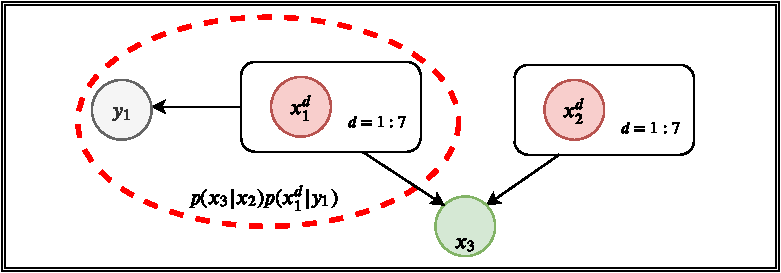
\includegraphics[width=0.4\textwidth]{parasite_model.pdf}
    \caption{The DAG of the Parasite model.}
  % \end{wrapfigure}
  \end{figure}
The parasite model by Smith el al.~\cite{smith2006relationship} is a simple stochastic 
model for determining the number of infections within a given population demographic.
The models hypothesised in ~\cite{smith2006relationship} were found, 
after extensive testing and development, to not characterise well the number 
of infections among different demographics, especially those under 15 years old. 
By using probabilistic programming we can immediately understand 
the expressiveness of the proposed model and can exact important insights for 
extending the proposed models, which increases ones ability to develop 
improved models to estimate parasite densities, given 
our observations of the seasonal entomological inoculation rate (EIR).
In addition to this we can greatly reduce the computational costs, whilst
improving model comprehension and expressivity.  
Although a statistical model is not formally defined within~\cite{smith2006relationship}
we define the unknown \emph{disease dynamics} parameters with a set of latent variables$\{x_{i}\}^{N}$
and construct the model as follows: 

\begin{align}
  \mu_i &= N \\ % pop size
  % disease dynamics
  S_{\infty} &\sim \mathcal{N}(\mu_\infty, \sigma^{2}_\infty) \\
  E_{crit} &\sim \mathcal{N}(\mu_{crit}, \sigma^{2}_{crit}) \\
  S_{imm} &\sim \mathcal{N}(\mu_{imm}, \sigma^{2}_{imm}) \\
  X_{p_{crit}} &\sim \mathcal{N}(\mu_{p_{crit}}, \sigma^{2}_{p_{crit}}) \\
  \gamma_p &\sim \mathcal{N}(\mu_{p}, \sigma^{2}_{p}) \\
  \rho_i & \sim \mathcal{U}(\mathbb{L}_i , \mathbb{U}_i) \\
  % integration for parasite densities in different demographics
  for \hspace{0.1cm} t &= 1:t_{max}: \\
  E_a &= \frac{E_{{max}_t}}{A_{max}} \times h_{\mu_{SA}}() \\
  X_p &= E_a + X_p \\
  S_1 &= S_{\infty} + \frac{(1 - S_\infty) }{1 + \frac{E_a}{E_{crit}}} \\
  S_2 &= S_{imm} + \frac{1 - S_{imm}}{1 + (\frac{X_p}{X_p_{crit}})^{\gamma_p}}\\
  %Probability of survival function
  S_p &= S_1 \times S_2 \\
  \lambda &= S_p \times E_a \\
  % Number of infections generated in unit time per individual sampled from poisson
  h &\sim Pos(\lambda) \\
  \texttt{if} &\hspace{0.1cm} h > 0: \\
  \hspace{2.3cm} &n_{infect} = 1 \\
  \text{TODO: add prevelance construction below}
  % % end for - add prevelance construction below
  % \mathcal{P}rev &= 
\end{align}

\textbf{TODO: Add some of the plots generated from this model and an accompanying analysis to them.}

\begin{wrapfigure}{l}{0.5\textwidth}
  \label{fig:amortized_sampling}
  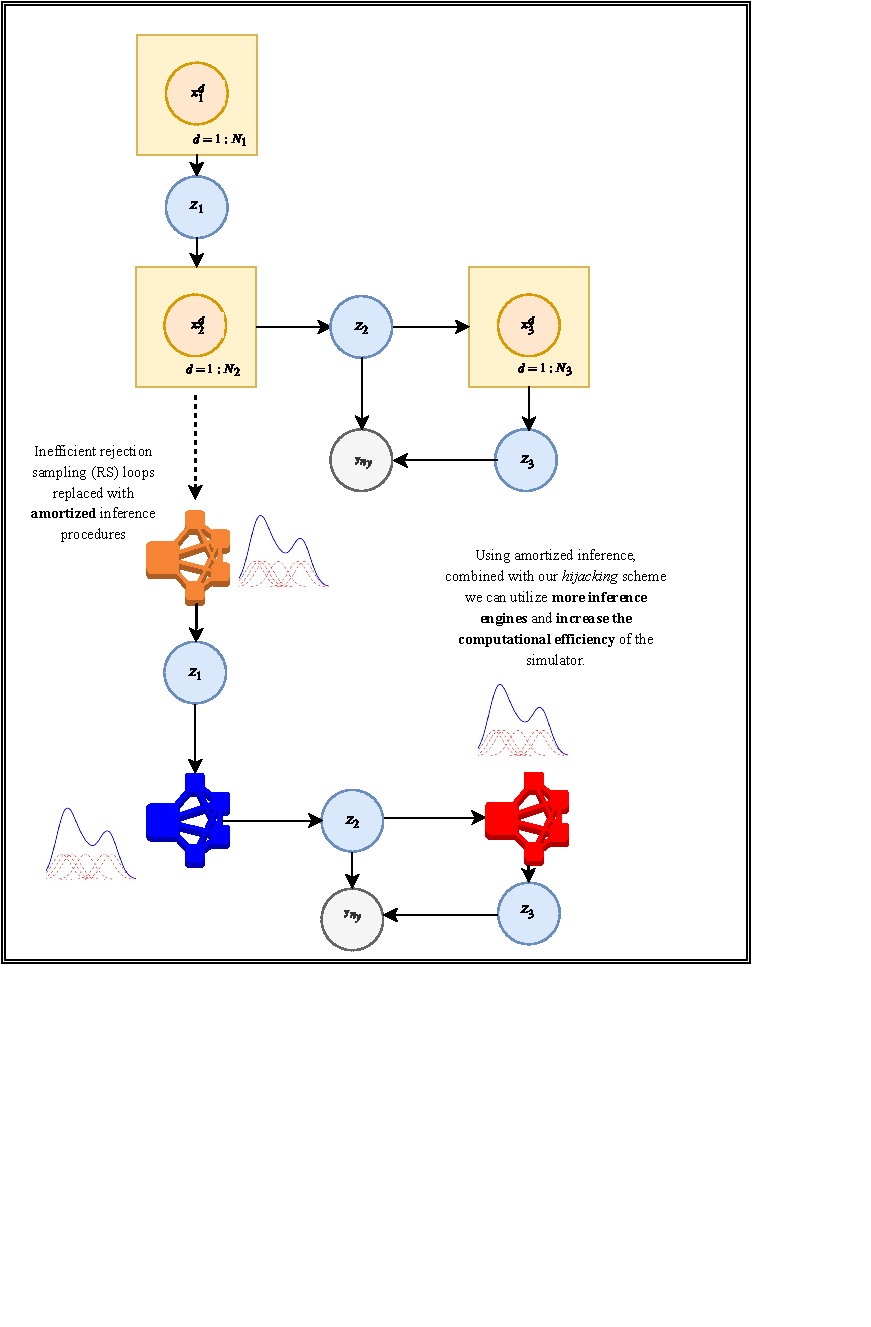
\includegraphics[width=0.5\textwidth,height=0.5\textheight]{amoritized_rejection.pdf}
  \vspace{-50pt}
  \caption{Using PyProb we can locate all regions of inefficient sampling 
  and replace those points in the code with learnt functions that represent
  the distributions of the rejection sampling statements. $Z_{i}$ represents the marginal and 
  by learning surrogate functions for each of the rejection sampling loops.
  In doing so we can learn approximate raw sample distributions $f(x_{i} | \eta)$ for each
  rejection sampling loop. This means that we can evaluate the function at each part in the simulator, enabling
  us to construct a target density that can be evaluated when using MCMC inference schemes such as RMH.
    }
  \end{wrapfigure}

\section{Additional TODOs}


\begin{itemize}
\item Before implementing such tools into the simulator, spend time looking for simpler stochastic simulators 
that can be hijacked but have target densities that can be constructed analytically. 
\item If we are not utilizing the additional information stored in the trace, which is only used during the inference compilation
training procedure, then we do not need it all, as for importance sampling we only require the weights after each \texttt{forward()}
update. 
\item If we cannot find any pre-existing simulators that are amenable to this approach then, we need to create our own, with
a rejection sampling loop, that can be exploited by the new machinery. This would enable us to debug, provide a simple example 
for the paper and understand the feasibility of the entire approach. 
\end{itemize}
\bibliographystyle{plain}
\bibliography{refs}

\end{document}